\documentclass{article}
\usepackage{graphicx} % Required for inserting images
\usepackage{wrapfig}
\usepackage{amsmath,amssymb,amsthm}
\usepackage{physics}
\usepackage{graphicx,float}
\graphicspath{{images/}}
\usepackage[none]{hyphenat}
\usepackage{blindtext}
\usepackage{parskip}
\usepackage[letterpaper,top=3cm, left= 3cm,bottom=3cm]{geometry}
\usepackage{subcaption}
\usepackage{tikz}
\usepackage{pgfplots}
\usepackage{esint}
\newcommand{\dbar}{d\hspace*{-0.08em}\bar{}\hspace*{0.1em}}
\pgfplotsset{compat=1.18}
\usetikzlibrary{positioning,calc,patterns,angles,quotes,shapes,plotmarks}
\numberwithin{equation}{section}

\title{Thermodynamic}
\author{Polaris}
\date{2025/08/17}

\begin{document}
\maketitle
\newpage
\tableofcontents
\newpage
\section{Basics}
\subsection{Kinetic Molecular Theory}
Kinetic Molecular theory states that gas is a bunch of always moving particles, the larger the temperature, the faster the particles is moving, the reason of this Brownian Motion. 

\subsection{Ideal Gas}
Ideal gas describes a type of gas where the gas particles do not interact with others, it follows the ideal gas law
\begin{equation}
    PV = Nk_BT = nRT
\end{equation}
Where $N$ is the number of gas particles, $k_B$ is the Boltzmann constant, $n$ is the amount of gas particles in moles, $R$ is the ideal gas constant, $T$ is the temperature of the gas.

\subsubsection{Average Kinetic Energy}
Average kinetic energy of a particles is related to the temperature as such
\begin{equation}
    \bar{K} = \frac{3}{2}k_BT
\end{equation}
Where $k_B$ is the Boltzmann constant, this can be derived through the maxwell distribution
\begin{equation}
    f(v) = 4\pi v^2 \left(\frac{m}{2\pi kT}\right)^{3/2} \exp{-\frac{mv^2}{2kT}}
\end{equation}
$f(v)$ is a probability density function which describes the probability of a particles having a velocity of $v$.

It can also be derived through the following model, consider a box full of gas particless of mass $m$ randomly moving, a piston with a side area of $S$ is located at the side of a box, a force of $F_{tot}$ is exerted on the piston to keep it in balance.

The pressure of the gas exerted on the piston is therefore
\[
P = \frac{F_{tot}}{S}
\]
\begin{figure}[h]
\centering
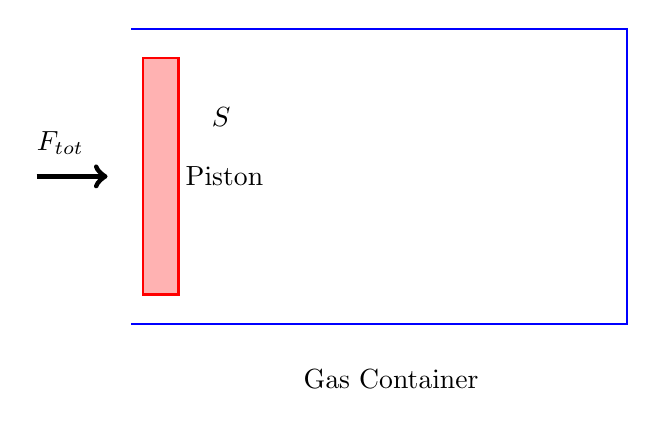
\begin{tikzpicture}[scale=1.5]
    % 定义主要尺寸
    \def\boxwidth{4}
    \def\boxheight{2.5}
    \def\pistonwidth{0.3}
    \def\pistonheight{2}
    
    % 画盒子主体(开口向左的长方形)
    \draw[thick, blue] 
        (0, 0) -- (\boxwidth, 0) -- 
        (\boxwidth, \boxheight) -- (0, \boxheight);
    
    % 画盒子的底部和顶部延伸(形成开口)
    \draw[thick, blue] (0, 0) -- (-0.2, 0);
    \draw[thick, blue] (0, \boxheight) -- (-0.2, \boxheight);
    
    % 画活塞(不同颜色的长方形)
    \fill[red!30] (-0.1, {\boxheight/2 - \pistonheight/2}) 
        rectangle ({\pistonwidth - 0.1}, {\boxheight/2 + \pistonheight/2});
    \draw[thick, red] (-0.1, {\boxheight/2 - \pistonheight/2}) 
        rectangle ({\pistonwidth - 0.1}, {\boxheight/2 + \pistonheight/2});
    
    % 活塞右侧的箭头
    \draw[->, line width=2pt] 
        (-{\pistonwidth - 0.7}, {\boxheight/2})--(-{\pistonwidth -0.1}, {\boxheight/2});
    
    \node[above] at (-{\pistonwidth - 0.5}, {\boxheight/2+0.1}) {$F_{tot}$};
    % 标注活塞面积S
    \node[right] at ({\pistonwidth + 0.1}, {\boxheight/2 + 0.5}) {$S$};
        
    % 标注
    \node[below] at ({\boxwidth/2}, -0.3) {Gas Container};
    \node[left] at (1, {\boxheight/2}) {Piston};
    
\end{tikzpicture}
\caption{A gas container with a piston on one side}
\end{figure}
By impulse theorem
\[
F\Delta t = 2mv_x
\]
Where $v_x$ is the velocity of the particle on $x$ axis, in a time period $t$, there are $N_1$ particles that hits the piston, therefore
\[
N_1 F\Delta t = F_{tot} t
\]
Substitute this in and define number density of particles as $N = nV$, one get 
\[
F_{tot} t = 2nV_1 mv_x
\]
Here $V_1$ is the volume of the particles that can hit the piston in time $t$, $V_1 = v_x t S$, therefore
\[
F_{tot} t = 2n v_x t S mv_x
\]
The pressure $P = F/S$ is
\[
P = 2nmv_x^2
\]
The velocity of different particle is different, therefore the total pressure is obtained by taking the average of velocity, at any moment, only half of the particle is moving towards the piston, therefore $\bar{v_x^2} = 1/2 v_x^2$
\[
P = nm\bar{v_x^2}
\]
The average velocity of gas particles on each axis is the same, therefore $\bar{v_x^2} = \bar{v_y^2} = \bar{v_z^2}$, hence pressure can be expressed as
\begin{equation}
    P = \frac{1}{3}nm\bar{v^2}
\end{equation}
Substitute this into the ideal gas law, the average kinetic energy of a gas particle is 
\begin{equation}
    \bar{E_k} = \frac{3}{2}k_BT
    \label{average EK}
\end{equation}
This is only valid for monatomic gas, for diatomic particles gas or triatomic gas, the average kinetic energy is 
\begin{equation}
    \bar{E}_k = \frac{i}{2}k_BT
    \label{general average KE}
\end{equation}
Where $i$ is the degree of freedom, for monatomic gas, $i=3$; for diatomic gas, $i=5$; for triatomic gas, $i=7$

\subsubsection{Internal Energy of Particles}
Internal energy is the sum of kinetic and potential energy of all particles in the gas
\[
U_{tot} = \sum_{n=1}^{i} E_i
\]
For an ideal gas, since there are no interaction between gas particle, poential energy is $0$, therefore the internal energy is the sum of all the kinetic energy of particles.
\begin{equation}
    U = \frac{3}{2}Nk_BT = \frac{3}{2}nRT
    \label{Ideal Gas Internal Energy}
\end{equation}
Where $N$ is the number of particles, generally
\[
U = \frac{i}{2}nRT
\]
Where $i$ is degree of freedom.
\subsection{Thermal Conduction}
Conduction is when 2 touching object transfer heat to each other (at least one of the object needs to be a solid)

The heat will transfer because heat is essentially viabration of particles, the faster viabrating one will impact the slower viabrating particles, which appears in the macro world as heat transfer.

A common theme is metal conducts heat faster than non metal, this is because metal tend to lose electron, the free electrons in the object will also conduct heat through its viabration. An expection is diamond, diamond conducts heat fast because the atoms are neatly arranged.

The equation that describes heat conduction is
\begin{equation}
    \frac{Q}{t} = kA\frac{\Delta T}{d}
\end{equation}
This is because heat conduction follows Fourier law
\begin{equation}
    \vec{q} = -k\nabla T
\end{equation}
Where $\vec{q}$ is the heat flux vector that points toward the cold object, when considering only one direction, the gradient can be written as a derivative. this results in the equation that describes the transfer of heat.
\begin{figure}[H]
    \centering
    \includegraphics[width=10cm]{pics/conduction.jpg}
    \caption{Heat conduction}
\end{figure}

\subsection{Thermal Expansion}
Thermal expansion follow a linear rule
\begin{equation}
    L = L_0 (1+\alpha \Delta T)
\end{equation}
$\alpha$ is known as the coefficient of thermal expansion, the expansion of volume follows the same rule
\[
V = V_0(1+\beta \Delta T)
\]
Where $\beta = 3\alpha$, this can be obtained through small value approximation.

\subsection{Thermal Radiation}
Radiation follows the Stefan-Boltzmann rule
\begin{equation}
    I = \varepsilon \sigma T^4
\end{equation}
Where $I$ is the intensity of the radiation, $\varepsilon$ is the emissivity, $\sigma$ is the Stefan-Boltzmann constant.

For a blackbody, $\varepsilon = 1$, this means a blackbody absords all energy it recieves and re-emit it as thermal radiation
\subsubsection{Example Question}
Consider 4 identical plane that can be seen as a blackbody, find $T_2$ and $T_3$ in terms of $T_1$ and $T_4$
\begin{figure}[H]
    \centering
    \begin{tikzpicture}
        \def\lineLength{4}
        \def\spacing{1.5}

        \foreach \i in {0,1,2,3} {
            \draw[thick] (\i*\spacing, 0) -- (\i*\spacing, \lineLength);
            \node[below] at (\i*\spacing, -0.2) {$T_{\the\numexpr\i+1\relax}$};
        }
    \end{tikzpicture}
\end{figure}
\textbf{Solution}: By conservation of energy, the energy recieved by the 2nd board is the same as the emergy it emits.
\[
    \begin{cases}
        A\sigma T_1^4 + A\sigma T_3^4 = 2A\sigma T_2^4\\
        A\sigma T_2^4 + A\sigma T_4^4 = 2A\sigma T_3^4
    \end{cases}
\]
The solution to this equation set is
\[
    \begin{cases}
        T_2 = \sqrt[4]{\dfrac{T_4^4 + 2T_1^4}{3}}\\
        T_3 = \sqrt[4]{\dfrac{T_1^4+2T_4^4}{3}}\\
    \end{cases}
\]
\newpage
\section{First Law of Thermodynamic}
The first law of thermodynamic is essentially conservation of energy, it states
\begin{equation}
    \boxed{Q = W + \Delta U}
    \label{FLOT}
\end{equation}
Where $Q$ is the heat absorbed by the gas, $W$ is the work done by the gas to the outside environment, $\Delta U$ is the change in internal energy.

The work done by the gas is related to the change of volume of gas and pressure of gas
\begin{equation}
    W = \int P dV
\end{equation}
Consider a chamber filled with ideal gas with a volume of $V$ and pressure of $P$, the gas expanded and gain a volume of $\Delta V$
\begin{figure}[H]
    \centering
    \includegraphics[width=10cm]{pics/gaswork.png}
    \caption{Expanding ideal gas}
\end{figure}
The work done is therefore 
\[
W = F\Delta x = PA \Delta x = P\Delta V
\]
If the gas expands, the work done by the gas is positive; if the gas contract, the work done by the gas is negative.

\subsection{Quasistatic Process and PV diagram}
Quasistatic process are process that is infintely slow to a point that every moment, the system is at equilibrium, it is a good approximation to approximate the change of gas.

Since the gas is always at equilibrium, the process is reversible. One can plot the property of gas in a PV diagram.
\begin{figure}[H]
    \centering
    \includegraphics[width=8cm]{pics/PVdiagram.png}
    \caption{PV diagram of a cycle}
\end{figure}
There are 2 advantages of PV diagram
\begin{enumerate}
    \item The highlighted area is the work done by the gas
    \item The isothermal line can be easily drawn, $PV \propto T$
\end{enumerate}
\subsection{Heat Capacity}
Heat capacity is a quantity that describes the relation betwen the amount of heat an object absorbed and the change of temperature
\begin{equation}
    C = \frac{dQ}{dT}
    \label{HC}
\end{equation}
During phase change, $C$ is infinite, this is because the temperature does not change in phase change while the object keeps absorbing heat.
\subsubsection{Isochoric Heat Capacity}
Isochoric heat capacity is the most important heat capacity, under a constant volume, it describes the relation between $Q$ and $T$, by first law of thermodynamic (equation \ref{FLOT})
\[
C_V = \frac{\Delta W + \Delta U}{\Delta T}
\]
For a isochoric process, $\Delta W = 0$, since the gas did not contract or exapnd, by equation \ref{Ideal Gas Internal Energy}, the isochoric heat capacity for ideal gas is
\begin{equation}
    \boxed{C_V = \frac{3}{2}nR}
\end{equation}
Where $n$ is the number of moles, generally, isochoric heat capacity is related to degree of freedom $i$
\[
C_V = \frac{i}{2}nR
\]

Molar Isochoric Heat Capacity is defined as the heat capacity for a mole of mass, for a monatomic gas, the molar isochoric heat capacity is 
\begin{equation}
    C_V = \frac{3}{2}R
\end{equation}
\subsubsection{Specific Heat Capacity}
Specific Heat Capacity refers to the amount of heat needed to raise the temperature of a object with a unit mass, it is defined as
\begin{equation}
    c = \frac{Q}{m\Delta T}
    \label{SHC}
\end{equation}
Where $m$ is the mass of the object, for ideal gas, this number is not a constant, consider a cycle of ideal gas. Assume that the specific heat capacity for a ideal gas is a constant.
\begin{figure}[H]
    \centering
    \includegraphics[width=8cm]{pics/idealgasSHC.png}
    \caption{A cycle completed by ideal gas}
\end{figure}
The area enclosed is clearly positive, therefore the gas had done work to the outside environment, the change in interal energy is $0$, therefore by first law of thermodynamic (equation \ref{FLOT}), the heat absorbed is larger than $0$.

By the definition of specific heat capacity (equation \ref{SHC}), the change in temperature is $0$, therefore the gas should not absorb heat, which contradicts the claim above, this means the specific heat capacity of an ideal gas is not a constant.

\subsection{Thermodynamic Process}
\subsubsection{Isobaric Process}
This process means that the pressure of gas is a constant, by ideal gas law
\begin{equation}
    \boxed{PV^0 = C}
\end{equation}
The work done in an isobaric process is 
\begin{equation}
    W = P_0 \Delta V
\end{equation}
By first law of thermodynamic, the relation between heat absorbed and change in volume is
\begin{align*}
    dQ &= dW + dU\\
    &= P_0 dV + \frac{3}{2}nRdT\\
    &= P_0 dV + \frac{3}{2}nR \frac{P_0}{nR}dV\\
    \int dQ &= \frac{5}{2} P_0 \int_{V_i}^{V_f} dV\\
\end{align*}
Therefore the heat absorbed is directly related to the change in volume
\begin{equation}
    Q = \frac{5}{2}P_0 \Delta V
\end{equation}
Generally, the relation between heat absorbed and volume change is
\[
Q = \frac{i}{2}P_0\Delta V
\]
Where $i$ is the degree of freedom. On a PV diagram, isobaric process is a horizontal line.
\begin{figure}[H]
    \centering
    \includegraphics[width=8cm]{pics/PVisobaric.jpg}
    \caption{Isobaric process in PV diagram}
\end{figure}
\subsubsection{Isochoric Process}
Isochoric process refers to a process where volume of gas is constant, which means no work is done on the gas, the heat absorb is directly related to the change in internal energy. By ideal gas law
\begin{equation}
    \boxed{PV^\infty = C}
\end{equation}
Therefore the absorb heat is proportional to the change in temperature
\[
\Delta Q = \frac{3}{2}nR \Delta T
\]
\subsubsection{Isothermal Process}
Isothermal process refers to a process where gas maintains a constant temperature, since internal energy $U\propto T$, constant temperature means no change in internal energy. By ideal gas law
\begin{equation}
    \boxed{PV = C}
\end{equation}
Where $C$ is a constant.

By first law of thermodynamic, the heat absorbed is equal to the work done by the gas.
\[
Q = W = \int_{V_1}^{V_2}PdV
\]
By ideal gas law, this integral can be written into
\begin{equation}
    W = nRT \int_{V_i}^{V_f} \frac{dV}{V} = nRT \ln{\left(\frac{V_f}{V_i}\right)}
\end{equation}
On a PV diagram, this process is a hyperbola connecting the initial state $(P_i, V_i)$ and final state $(P_f , V_f)$ of the gas.
\begin{figure}[H] 
    \centering
    \includegraphics[width=8cm]{pics/PVisothermal.png}
    \caption{PV diagram of isothermal process}
\end{figure}
One can see that if $V_f > V_i$, the gas do positive work to the outside environment; if $V_f < V_i$, the gas do negative work to the outside environment (or outside environment does positive work)
\subsubsection{Adiabatic Process}
Adiabatic process refers to a process where the gas does not absorb heat from external environment, therefore the change in internal energy is solely due to the work done by the gas.
\[
W = -\Delta U
\]
Take differential on both side of ideal gas law
\[
    PdV + VdP = nRdT\\
\]
The change in temperature is related to the change in internal energy by $dU = C_V dT$, this is because the change in internal energy is equivalent to absorbing heat in an isochoric process. Therefore the relation can be turned into
\begin{align*}
    PdV + VdP &= -nR \frac{PdV}{C_V}\\
    PdV \left(1+\frac{nR}{C_V}\right) &= -VdP\\
\end{align*}
Denote $\gamma = 1+ \dfrac{nR}{C_V} = \dfrac{C_V + nR}{C_V} = \dfrac{i+2}{i}$ as the \textbf{adiabatic index}, where $i$ is the degree of freedom, the equation turns into
\begin{align*}
    \gamma PdV &= -VdP\\
    \gamma \frac{dV}{V} &= - \frac{dP}{P}\\
    \ln{\left(\frac{V_i}{V_f}\right)^\gamma} &= \ln\left(\frac{P_f}{P_i}\right)\\
\end{align*}
Therefore for an adiabatic process
\begin{equation}
    \boxed{PV^\gamma = C}
\end{equation}
Where $C$ is a constant, For a monatomic ideal gas, $\gamma = 5/3$, for photon gas, $\gamma = 4/3$.

To find the work done by the gas, use the definition of work
\begin{align*}
    W &= \int_{V_i}^{V_f} PdV\\
    &= \int_{V_i}^{V_f} \frac{C}{V^\gamma} dV\\
    &= \frac{K}{1-\gamma} \left(V_2^{1-\gamma} - V_1^{1-\gamma}\right)\\
    &= \frac{PV^\gamma}{1-\gamma} \left(V_2^{1-\gamma} - V_1^{1-\gamma}\right)\\
\end{align*}
Therefore the work done by the gas is
\begin{equation}
    W = \frac{P_f V_f - P_i V_i}{1-\gamma}
\end{equation}
On PV diagram, adiabatic process can be represented as such (the two gray lines are isothermal lines).
\begin{figure}[H]
    \centering
    \includegraphics[width=8cm]{pics/PVadiabatic.png}
    \caption{Adiabatic process on PV diagram}
\end{figure}

\newpage
\section{Second Law of Thermodynamic}
A heat engine is basically a machine that absorbs heat and do work.
\begin{figure}[H]
    \centering
    \includegraphics[width=4cm]{pics/heatenginediagram.png}
    \caption{Schematic Diagram of Heat Engine}
\end{figure}
Such example include a car engine.
\begin{figure}[H]
    \centering
    \includegraphics[width=12cm]{pics/engine.png}
    \caption{Engine cycle}
\end{figure}
The engine draws heat from the hot gas and convert it into work and some cold heat.

\subsection{Entropy in a quasistatic cycle}
Define entropy as
\begin{equation}
    dS = \oint \frac{\dbar Q}{T}
\end{equation}
Where $\dbar$ is a small increase in heat, this is known as a process quantity, it is dependent on the specific process it takes; on the contrary is state quantity, which is only dependent on the initial and final state. For example work done by gravity is state quantity and work done by friction is process quantity.

In a quasistatic cycle process, entropy does not change, from first law of thermodynamic
\[
\dbar Q = dU + PdV
\]
Divide both side by $T$ and substitute $dU = C_V dT$ (equation \ref{HC})
\[
\frac{\dbar Q}{T} = C_V \frac{dT}{T} + \frac{PdV}{T}
\]
For a cycle, $dT=0$ and $dV=0$, therefore the integral over this cycle is also $0$, hence 
\begin{equation}
    dS = \oint\frac{\dbar Q}{T} = 0
    \label{cycledS}
\end{equation}
\subsection{Efficiency of Heat engine}
Define efficiency of heat engine as the quotient between the work done and the heat absorb.
\begin{equation}
    \eta = \frac{W}{Q_H} = 1 - \frac{Q_L}{Q_H}
\end{equation}
Where $Q_H$ is the heat absorbed from the high temperature source, $Q_L$ is the heat released to the low temperature source.
\subsection{Carnot Cycle}
Carnot Cycle is the most efficient thermodynamic cycle, it is composed of 2 isothermal process and 2 adiabatic process. 

A heat engine that preforms the Carnot cycle is called a Carnot engine, no real Carnot engine exist because no real adiabatic process exist and no real quasistatic process exist.

The gas first preform isothermal expansion, which extract heat from high temperature source and do work to the outside environment, then the gas preform adiabatic expansion to cool down, then the gas preform isothermal contraction to take in heat and store energy, then preform adiabatic contraciton to raise temperature for the next cycle.
\begin{figure}[H]
    \centering
    \includegraphics[width=10cm]{pics/carnotpv.png}
    \caption{PV diagram of Carnot Cycle}
\end{figure}
\subsubsection{Efficiency of Carnot Cycle}
By the definition of efficiency, efficiency can be obtained through $Q_H$ and $Q_L$. Since adiabatic process does not involve heat, the only factor to consider is the isothermal process.

The absolute value of heat absorbed/released in Carnot Cycle is 
\[
Q = nRT\ln{\frac{V_f}{V_i}}
\]
Therefore
\[
Q_H = nRT_H \ln \frac{V_b}{V_a} \text{ and } Q_L = nRT_L \ln \frac{V_c}{V_d}
\]
Here $V_c$ is at the numerator despite it is the initial state is because it is taking the absolute value of $Q_L$ here, to find the actual value, $V_c$ is at denominator.

Since bc and ad are also connected through a adiabatic process, the relation between volume and temperature can also be used to find the relations between different volume ($TV^{\gamma - 1} = C$). Therefore
\[
\frac{T_d}{T_a} = \frac{V_a^{\gamma-1}}{V_d^{\gamma-1}} \text{ and } \frac{T_b}{T_c} = \frac{V_c^{\gamma-1}}{V_b^{\gamma-1}}
\]
Since $T_c = T_d$ and $T_a = T_b$, the relationship between volume is obtained
\[
\frac{V_b}{V_a} = \frac{V_c}{V_d}
\]
Therefore the efficiency of Carnot engine is
\begin{equation}
    \eta = 1 - \frac{T_L}{T_H}
\end{equation}
This efficiency can also be found through using equation \ref{cycledS}, for a isothermal process 
\[
dS_{ab} = \int_{a}^{b} \frac{\dbar Q}{T} = \frac{Q_H}{T_H} \text{ and } dS_{cd} = \int_{c}^{d} \frac{\dbar Q}{T}= \frac{Q_L}{T_L}
\]
In a adiabatic process, no heat is exchanged, therefore $dS = 0$, since integrating this over a cycle yields a result of $0$
\[
\frac{\abs{Q_H}}{T_H} = \frac{\abs{Q_L}}{T_L}
\]
Therefore the efficiency of Carnot engine can be easily found.

\newpage
\subsection{Otto Cycle}
Otto Cycle is the most common cycle in car engine, it is composed of 2 adiabatic cycle and 2 isochoric cycle.
\begin{figure}[H]
    \centering
    \includegraphics[width=10cm]{pics/ottoCycle.png}
    \caption{PV diagram of Otto Cycle}
\end{figure}
\subsubsection{Efficiency of Otto Cycle}
In adiabatic process, no heat is absorbed or released, therefore the heat absorbed and released is only dependent on the isochoric process.

The heat released by a isochoric process is 
\[
Q_{in} = \frac{3}{2}nR (T_4 - T_1) \text{ and } Q_{out} = \frac{3}{2}nR (T_3 - T_2)
\]
At the same time, adiabatic process gives
\[
\frac{T_1}{T_2} = \frac{T_3}{T_4} = \left(\frac{V_{max}}{V_{min}}\right)^{\gamma - 1}
\]
Therefore the efficiency of the Otto cycle is
\[
\eta = 1 - \frac{Q_{out}}{Q_{in}} = 1- \frac{T_3 - T_2}{T_1-T_4}
\]
Here we switch the orders between $T_1$ and $T_4$ because $T_1 > T_4$. Therefore the efficiency in terms of volume is
\begin{equation}
    \eta = 1 - \left(\frac{V_{min}}{V_{max}}\right)^{\gamma}
\end{equation}
\newpage
\section{Second Law of Thermodynamic}
There are 2 equivalent expression for Second Law of Thermodynamic, the Clausius Statement and Kelvin Statement

Clausius Statement: Heat can never pass from a colder to a warmer body without some other change, connected therewith, occurring at the same time.

Kelvin Statement: It is impossible for a self-acting machine to absorb heat from one source and turn all absorbed heat into work.

The two expression are equivalent, here is the proof.

\begin{enumerate}
    \item Kelvin to Clausius:
    
    Assume the Kelvin Statement is true and the Clausius Statement is false, one can construct a heat engine where the heat transfer to the lower temperature source will flow back to the high temperature source.

    Assume a heat of $Q_H$ is absorbed by the heat engine, a heat of $Q_L$ is transferred to the lower temperature source and then absorbed by the high temperature source. This is equivalent to high temperature source absorbing a heat of $Q_H-Q_L$ and turning everything into work. Which violates the Kelvin Statement.

    \item Clausius to Kelvin
    
    Assume that Clausius Statement is true and Kelvin Statement is false, one can construct a cooling device with $\eta = 1$, it absorbs a heat of $Q_L$ from low temperature source and turn all of it into work $W$. Then one can construct a machine that converts all the work into heat and transfer it into a high temperature source. If the two machine is working together, it appears that heat is going from low temperature to high temperature, which violates the Clausius statement.
\end{enumerate}
Here we proved that the two statement cannot be one true one false at the same time, therefore they are equivalent to each other.

\subsection{Entropy}
Define \textbf{entropy} as
\begin{equation}
    \dbar S = \oint \frac{dQ}{T}
\end{equation}
Entropy is only a conserved quantity when the thermodynamic process is reversible. This is because a reversible process means no net released heat. For a irreversible process, entropy only increase.
\end{document}